%% Based on a TeXnicCenter-Template by Gyorgy SZEIDL.
%%%%%%%%%%%%%%%%%%%%%%%%%%%%%%%%%%%%%%%%%%%%%%%%%%%%%%%%%%%%%

%------------------------------------------------------------
%
\documentclass[landscape,twoside]{article}%
%Options -- Point size:  10pt (default), 11pt, 12pt
%        -- Paper size:  letterpaper (default), a4paper, a5paper, b5paper
%                        legalpaper, executivepaper
%        -- Orientation  (portrait is the default)
%                        landscape
%        -- Print size:  oneside (default), twoside
%        -- Quality      final(default), draft
%        -- Title page   notitlepage, titlepage(default)
%        -- Columns      onecolumn(default), twocolumn
%        -- Equation numbering (equation numbers on the right is the default)
%                        leqno
%        -- Displayed equations (centered is the default)
%                        fleqn (equations start at the same distance from the right side)
%        -- Open bibliography style (closed is the default)
%                        openbib
% For instance the command
%           \documentclass[a4paper,12pt,leqno]{article}
% ensures that the paper size is a4, the fonts are typeset at the size 12p
% and the equation numbers are on the left side
%
\usepackage[T1]{fontenc}
\usepackage{amsmath}%
\usepackage{amsfonts}%
\usepackage{amssymb}%
\usepackage{graphicx}
\usepackage{multicol}
\usepackage[landscape]{geometry}
\usepackage{algorithm}
\usepackage{algpseudocode}
\usepackage{tabularx}
\usepackage[mono=false]{libertine}
\usepackage[mathscr]{euscript}
\usepackage{enumitem}
\usepackage{caption}
%-------------------------------------------
\newtheorem{theorem}{Theorem}
\newtheorem{acknowledgement}[theorem]{Acknowledgement}
\newtheorem{axiom}[theorem]{Axiom}
\newtheorem{case}[theorem]{Case}
\newtheorem{claim}[theorem]{Claim}
\newtheorem{conclusion}[theorem]{Conclusion}
\newtheorem{condition}[theorem]{Condition}
\newtheorem{conjecture}[theorem]{Conjecture}
\newtheorem{corollary}[theorem]{Corollary}
\newtheorem{criterion}[theorem]{Criterion}
\newtheorem{definition}[theorem]{Definition}
\newtheorem{example}[theorem]{Example}
\newtheorem{exercise}[theorem]{Exercise}
\newtheorem{lemma}[theorem]{Lemma}
\newtheorem{notation}[theorem]{Notation}
\newtheorem{problem}[theorem]{Problem}
\newtheorem{proposition}[theorem]{Proposition}
\newtheorem{remark}[theorem]{Remark}
\newtheorem{solution}[theorem]{Solution}
\newtheorem{summary}[theorem]{Summary}
\newenvironment{proof}[1][Proof]{\textbf{#1.} }{\ \rule{0.5em}{0.5em}}


\newcommand{\overbar}[1]{\mkern 1.5mu\overline{\mkern-1.5mu#1\mkern-1.5mu}\mkern 1.5mu}


\geometry{top=0.5in, left=0.5in, right=0.5in, bottom=0.5in}

\pagestyle{empty}

% Redefine section commands to use less space
\makeatletter
\renewcommand{\section}{\@startsection{section}{1}{0mm}%
                                {-1ex plus -.5ex minus -.2ex}%
                                {0.5ex plus .2ex}%x
                                {\normalfont\large\bfseries}}
\renewcommand{\subsection}{\@startsection{subsection}{2}{0mm}%
                                {-1explus -.5ex minus -.2ex}%
                                {0.5ex plus .2ex}%
                                {\normalfont\normalsize\bfseries}}
\renewcommand{\subsubsection}{\@startsection{subsubsection}{3}{0mm}%
                                {-1ex plus -.5ex minus -.2ex}%
                                {1ex plus .2ex}%
                                {\normalfont\small\bfseries}}
\makeatother

\setcounter{secnumdepth}{0}

\setlength{\parindent}{0pt}
\setlength{\parskip}{0pt plus 0.5ex}

\setitemize{noitemsep, topsep=0pt, parsep=0pt, partopsep=0pt}
\setenumerate{noitemsep, topsep=0pt, parsep=0pt, partopsep=0pt}

\newcommand{\Break}{\textbf{break}}
\newcommand{\Var}[1]{\textsf{#1}}
\newcommand{\alg}[1]{\textsc{\bfseries \footnotesize #1}}

\begin{document}
\raggedright
\begin{multicols}{3}
\setlength{\premulticols}{1pt}
\setlength{\postmulticols}{1pt}
\setlength{\multicolsep}{1pt}
\setlength{\columnsep}{2pt}

\begin{center}
     \Large{\underline{Algorithms Final Cheat Sheet}} \\
\end{center}

\section{Randomized Algorithms}

\subsection{Processes and DB}
Assume each process $P_i$ has some probability $p$ to access a database. A successful round is when exactly one process accesses the database. The probability of a single successful round is $p(1 - p)^{n-1}$.\\
We can maximize this probability by setting $p = \frac{1}{n}$. The probability of success here is $\Theta(\frac{1}{n})$.\\
Now, let's examine how long it will take process $P_i$ to succeed in accessing the database at least once. Running $t$ times, the probability that process $P_i$ does not succeed in any of rounds 1 through $t$ is $\leq (1 - \frac{1}{en})^t$. Setting $t$ to $\left\lceil en \right\rceil$ means the probability is $\leq e^{-1}$, independent of $n$.\\
If we set $t = \left\lceil en \right\rceil \cdot (c \ln n)$, the probability of failure is upper-bounded by $n^{-c}$.\\
With probablity at least $1 - n^{-1}$, all processes succeed in accessing the database at least once within $t = 2 \left\lceil en \right\rceil \ln n$ rounds.

\subsection{The Union Bound}
Prob [ $\bigcup\limits_{i=1}^{\infty} F_{i}$ ] <= $\sum_{n=1}^{\infty}  Prob[ F_{i}] $ 

%%%%%%%

\subsection{Verifying AB=C}

B$\overbar{r} -> A(B\overbar{r})$ and $C\overbar{r}$. if $A(B\overbar{r}) != C\overbar{r}$ then $AB != C$

\subsection{Principle of Deferred Decisions}
If $AB != C$ and $\overbar{r}$ is chosen uniformly at random with $r_n$ at 0-1 then Prob($AB\overbar{r} = C\overbar{r}) <= 1/2$

\subsection{Law of Total Probability}
Let $E_1 ... E_n$ be mutually disjoint events in the sample space $\Omega$ and let $\bigcup\limits_{i=1}^{n} E_{i}$ then $\sum_{i=1}^{n}  Prob[ B | E_{i}] Prob[E_{i}] $ 

Repeated trials increase the runtime to $\Theta(kn^2)$
If it returns false, then it this is right, but if it returns true, then it returns so with some probability of mistake.

%%%%%%%

\subsection{Median Value}
$\sum_{j=1}^{\infty}  j * Prob[ X = j ]  = (n + 1) / 2$ while Prob $[X = j] = 1/n$

To take exactly $j$ steps: Prob $[X = j] = (1 - p)^{j - 1} p$
$1/p$ for the first success

\subsection{Median Value}
Linearity of Expectation: Given 2 random vars $X$ and $Y$ in the same probability space, $E [X + Y] = E[ X ] + E [ Y ] $

\subsection{Memoryless guessing}
Expected correct: 1, independent of $n$

\subsection{Memory guessing}
$H(n) = \Theta(log(n))$ [harmonic series]

\subsection{Coupon collection:}
$E[ X_{j}] = n / (n - j); n $= number of; $j$ = collected; $( n - j ) / n$ of getting a new one
$E[X] = nH(n) = \Theta(nlog(n))$

\subsection{Conditional Probability}
$E[ X | \alpha ] =  \sum_{j=0}^{\infty} j *$ Prob $[ X = j | \alpha]$

\subsection{Max 3-SAT}
There is a randomized algo with polynomial expected run time that is guaranteed to produce a truth assignment satisfying at least a $7/8$ fraction of all clauses. We would need $8k$ trials to get the satisfying assignment.

\begin{algorithmic}[1]
	\Function{Select}{$S, k$}
		\State {$a_i \gets random var in S$}
		\For{each element $a_j$ of $S$}
			\State{$S^{-}$.append($a_j$) if $a_j < a_i$}
			\State{$S^{+}$.append($a_j$) if $a_j > a_i$}
		\EndFor
		\If{$S^{-} = k - 1$}
			\State{return $a_i$}
		\ElsIf{$S^{-} \geq k$}
			\State{Select($S^{-}, k$)}
		\Else
			\State{Select($S^{+}, k-1- |S^{-}|$)}
		\EndIf
	\EndFunction
\end{algorithmic}

%%%%

\subsection{Quicksort ExpectedComparisons}
$2nln(n) + O(n), \Omega(nlogn)$

%%%

\subsection{Uniform}

Prob $[h(x) = i] = 1/m$ for all $x$ and all $i$

\subsection{Universal}
Prob $[h(x) = h(y)] = 1/m$ for all $x != y$
\subsection{Near-universal}
Prob $[h(x) = h(y)] \leq 2/m$ for all $x != y$; E[$chainLen$] $\leq 2*\alpha;$ Runtime: $\Theta(1 + \alpha)$
\subsection{k-uniform}
Prob $ [ \wedge{}_{j=1}^{k} h(x_j) = i_j) ] = 1 / m^{k}$ for all distinct $x_1...x_k$ and all $i_1...i_k$
\subsection{Load Factor}
$\alpha = n/m$
\subsection{Balanced Binary Tree Search}
O(1 + log($chainLen$)) with any hash 
O(1 + log($\alpha$)) for uniform
\subsection{Recursively Hash}
$O(log_{m}{n})$
\subsection{Expected Search w/ binary probe}
O(1)
MaxFlowsMinCuts
FlowCutApplications
\section{SAT and CNF-SAT}

\subsection{Formula Satisfiability/SAT}
Given a boolean formula like $(a \vee b \vee c \vee \overline{d}) \Leftrightarrow ((b \wedge \overline{c}) \vee \overline{ ( \overline{a} \Rightarrow d) } \vee (c \neq a \wedge b))$, is it possible to assign boolean values to $a, b, c, \ldots$ so that the formula evaluates to \Var{True}?\\

We can transform any boolean circuit to a formula in linear time (using depth-first search), and the size of the resulting formula is only a constant factor larger than the size of the circuit. Thus, we have a polynomial-time reduction from circuit satisfiability to SAT. Thus, SAT is NP-hard.\\

To prove that a boolean formula is satisfiable, we only have to specify an assignment to the variables that makes the formula \Var{True}. We can check the proof in linear time just by reading the formula from left to right, evaluating as we go. So SAT is also in NP, and thus is NP-complete.

\subsection{CNF}
A boolean form is in \emph{conjunctive normal form} if it is a conjunction (\alg{and}) of several clauses, each of which is the disjunction (\alg{or}) of several \emph{literals}, each of which is either a variable or its negation. For example, $(a \vee b \vee c \vee d) \wedge (b \vee \overline{c} \vee \overline{d}) \wedge (\overline{a} \vee c \vee d) \wedge (a \vee \overline{b})$.

\subsection{3CNF}
A 3CNF formula is a CNF formula with exactly 3 literals per clause; the previous example is not a 3CNF formula, since its first clause has four literals and its last clause has only two. 3SAT is just SAT restricted to 3CNF formulas: Given a 3CNF formula, is there an assignment to the variables that makes the formula evaluate to \Var{True}?

\begin{enumerate}
	\item Make sure every \alg{and} and \alg{or} gate has only two inputs. If any gate has $k > 2$ inputs, replace it with a binary tree of $k - 1$ two-input gates.
	\item Write down the circuit as a formula, with one clause per gate.
	\item Change every gate clause into a CNF formula
	\item Make sure every clause has exactly three literals
\end{enumerate}

Every binary gate in the original circuit will be transformed into at most 5 clauses.
\section{NP-Hardness}
\begin{definition}
\emph{P} is the set of decision problems that can be solved in polynomial time. Intuitively, P is the set of problems that can be solved quickly.
\end{definition}
\begin{definition}
\emph{NP} is the set of decision problems with the following property: if the answer is \Var{Yes}, then there is a \emph{proof} of this fact that can be checked in polynomial time. Intuitively, NP is the set of decision problems where we can verify a \Var{Yes} answer quickly if we have the solution in front of us.
\end{definition}
\begin{definition}
\emph{co-NP} is essentially the opposite of NP. If the answer to a problem in co-NP is \Var{No}, then there is a proof of this fact that can be checked in polynomial time.
\end{definition}
Every decision problem in P is also in NP and also in co-NP.
\begin{definition}
A problem $\Pi$ is \emph{NP-hard} if a polynomial-time algorithm for $\Pi$ would imply a polynomial-time algorithm for every problem in NP.
\end{definition}
\begin{definition}
A problem $\Pi$ is \emph{NP-complete} if it is both NP-hard and an element of NP.
\end{definition}
\begin{theorem}[Cook-Levin Theorem]
Circuit satisfiability is NP-complete.
\end{theorem}
To prove that problem $A$ is NP-hard, reduce a known NP-hard problem to $A$.
\begin{definition}
A \emph{many-one} reduction from one language $L' \subseteq \Sigma^*$ is a function $f : \Sigma^* \rightarrow \Sigma^*$ such that $x \in L'$ iff $f(x) \in L$. A \emph{language} $L$ is NP-hard iff, for any language $L' \in NP$, there is a \emph{many-one} reduction from $L'$ to $L$ that can be computed in polynomial time.
\end{definition}
\subsection{NP-Hard Problems}
\begin{itemize}
	\item SAT
	\item 3SAT
	\item Maximum Independent Set: find the size of the largest subset of the vertices of a graph with no edges between them
	\item Clique: Compute the number of nodes in its largest complete subgraph
	\item Vertex Cover: Smallest set of vertices that touch every edge in the graph
	\item Graph Coloring: Find the smallest possible number of colors in a legal coloring such that every edge has two different colors at its endpoints
	\item Hamiltonian Cycle: find a cycle that visits each vertex in a graph exactly once
	\item Subset Sum: Given a set $X$ of positive integers and an integer $t$, determine whether $X$ has a subset whose elements sum to $t$
	\item Planar Circuit SAT: Given a boolean circuit that can be embedded in the plane so that no two wires cross, is there an input that makes the circuit output \Var{True}
	\item Not All Equal 3SAT: Given a 3CNF formula, is there an assignment of values to the variables so that every clause contains at least one \Var{True} literal \emph{and} at least one \Var{False} literal?
	\item Exact 3-Dimensional Matching: Given a set $S$ and a collection of three-element subsets of $S$, called \emph{triples}, is there a sub-collection of disjoint triples that exactly cover $S$?
	\item Partition: Given a set $S$ of $n$ integers, are there subsets $A$ and $B$ such that $A \cup B = S$, $A \cap B = \emptyset$, and $\sum_{a \in A} a = \sum_{b \in B} b$?
	\item 3Partition: Given a set $S$ of $3n$ integers, can it be partitioned into $n$ disjoint three-element subsets, such that every subset has exactly the same sum?
	\item Set Cover: Given a collection of sets $\mathscr{S} = \{ S_1, S_2, \ldots, S_m \}$, find the smallest sub-collection of $S_i$'s that contains all the elements of $\bigcup_i S_i$
	\item Hitting Set: Given a collection of sets $\mathscr{S} = \{ S_1, S_2, \ldots, S_m \}$, find the minimum number of elements of $\bigcup_i S_i$ that hit every set in $\mathscr{S}$
	\item Hamiltonian Path: Given a graph $G$, is there a path in $G$ that visits every vertex exactly once?
	\item Longest Path: Given a non-negatively weighted graph $G$ and two vertices $u$ and $v$, what is the longest simple path from $u$ to $v$ in the graph? A path is \emph{simple} if it visits each vertex at most once.
	\item Steiner Tree: Given a weighted, undirected graph $G$ with some of the vertices marked, what is the minimum-weight subtree of $G$ that contains every marked vertex?
\end{itemize}

\subsection{Hamiltonian Cycle [From Vertex Cover]}

For each vertex $u$, all the edge gadgets are connected in $H$ into a single directed path, a vertex chain. $H$ has $d-1$ additional edges for each $i$. $H$ also contains $k$ cover vertices, $1 - k$, with a directed edge to the first vertex in each vertex chain and a directed edge from the last vertex in each vertex chain.\\

Start at cover vertex 1 and traverse vertex chain for $vu_{2}$, then visit cover vertex 2 and so on and so forth before returning to 1. If $v$ is a part of the vertex cover, follow the edge from $(u_{i}, v, in)$ to $(u_{i}, v, out)$, else, detour from  $(u_{i}, v, in)$ > $(v, u_{i}, in)$ > $(v, u_{i}, out)$ > $(u_{i}, v, out)$.\\

$G$ contains a vertex cover of size $K$ if and only if $H$ contains a Hamiltonian cycle

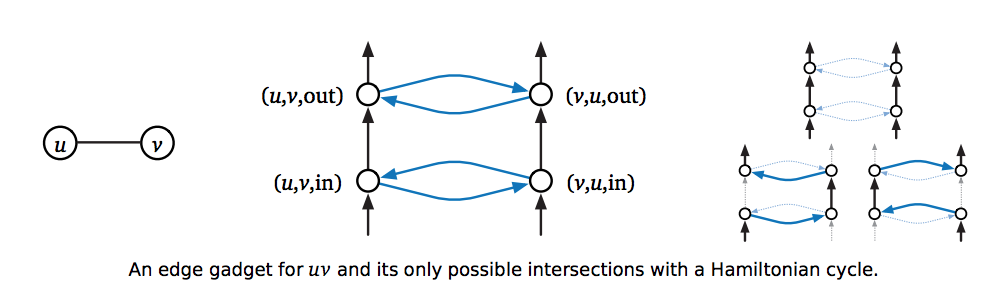
\includegraphics[width=\linewidth]{images/edgegadget.png}
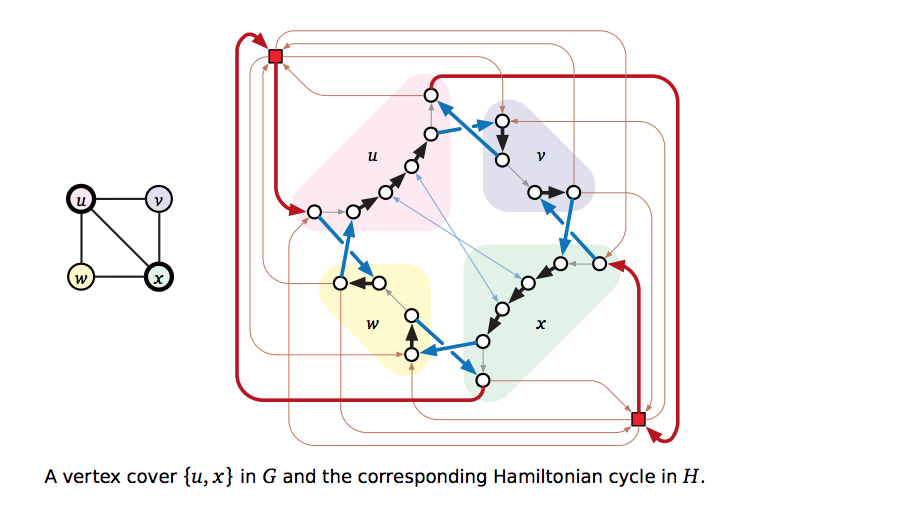
\includegraphics[width=\linewidth]{images/hamiltoniancycle.png}

\subsection{Subset Sum}

Given a graph $G$ and an integer $k$, first number edges from 0 to $m-1$; set $X$ contains the integer $b_{i} = 4^{i}$ for each edge $i$, and the integer $a_{v} = 4^{m} + \sum_{i \in \delta(v)}{4^i}$ where $\delta(v)$ is the set of edges that have $v$ as an endpoint. Finally, we set the target sum: $t = k * 4^m + \sum_{i = 0}^{m-1}{2 * 4^i}$

\subsection{LIS -> DAG}

Turn every number in the sequence into a vertex in a graph. Construct a special vertex $d$. For each vertex $v_1$, construct an edge to another vertex $v_2$ if (1) $v_2$ comes after $v_1$ in the sequence, and (2) $v_2$ > $v_1$. Also construct an edge to $d$.\\ 

Every path on this graph is a valid increasing subsequence. The problem of finding the LIS is now the problem of finding the longest path on this graph. Apply DAG.

\end{multicols}
\end{document}
